\documentclass[class=NCU_thesis, crop=false]{standalone}
\begin{document}

\chapter{前言}
這是一個簡易的\LaTeX\ 教學。概略的介紹\LaTeX\ 的用法,並且使用Cookbook的形式寫作。也就是說使用者可以直接複製/貼上\LaTeX\ code ,省去慢慢打、慢慢學的時間。除了\LaTeX\ 語法外,本文也會介紹一些幫助撰寫\LaTeX\ 的工具。所有知識都不會說的太詳細,各位要深入了解的話就請各位自行發揮舉一反三的能力上Google搜尋囉!
這份文件(以及論文樣板)歡迎各位自由使用、修改、發佈。發現內容有誤也歡迎指正。
如果研究生認為我幫你節省很多時間,想感謝一下的話,請推薦更多人閱讀、採用,這樣就可以稀釋我的時間成本了QQ 。

\tikz[remember picture,overlay] \node[opacity=0.1,inner sep=0pt] at (current page.center){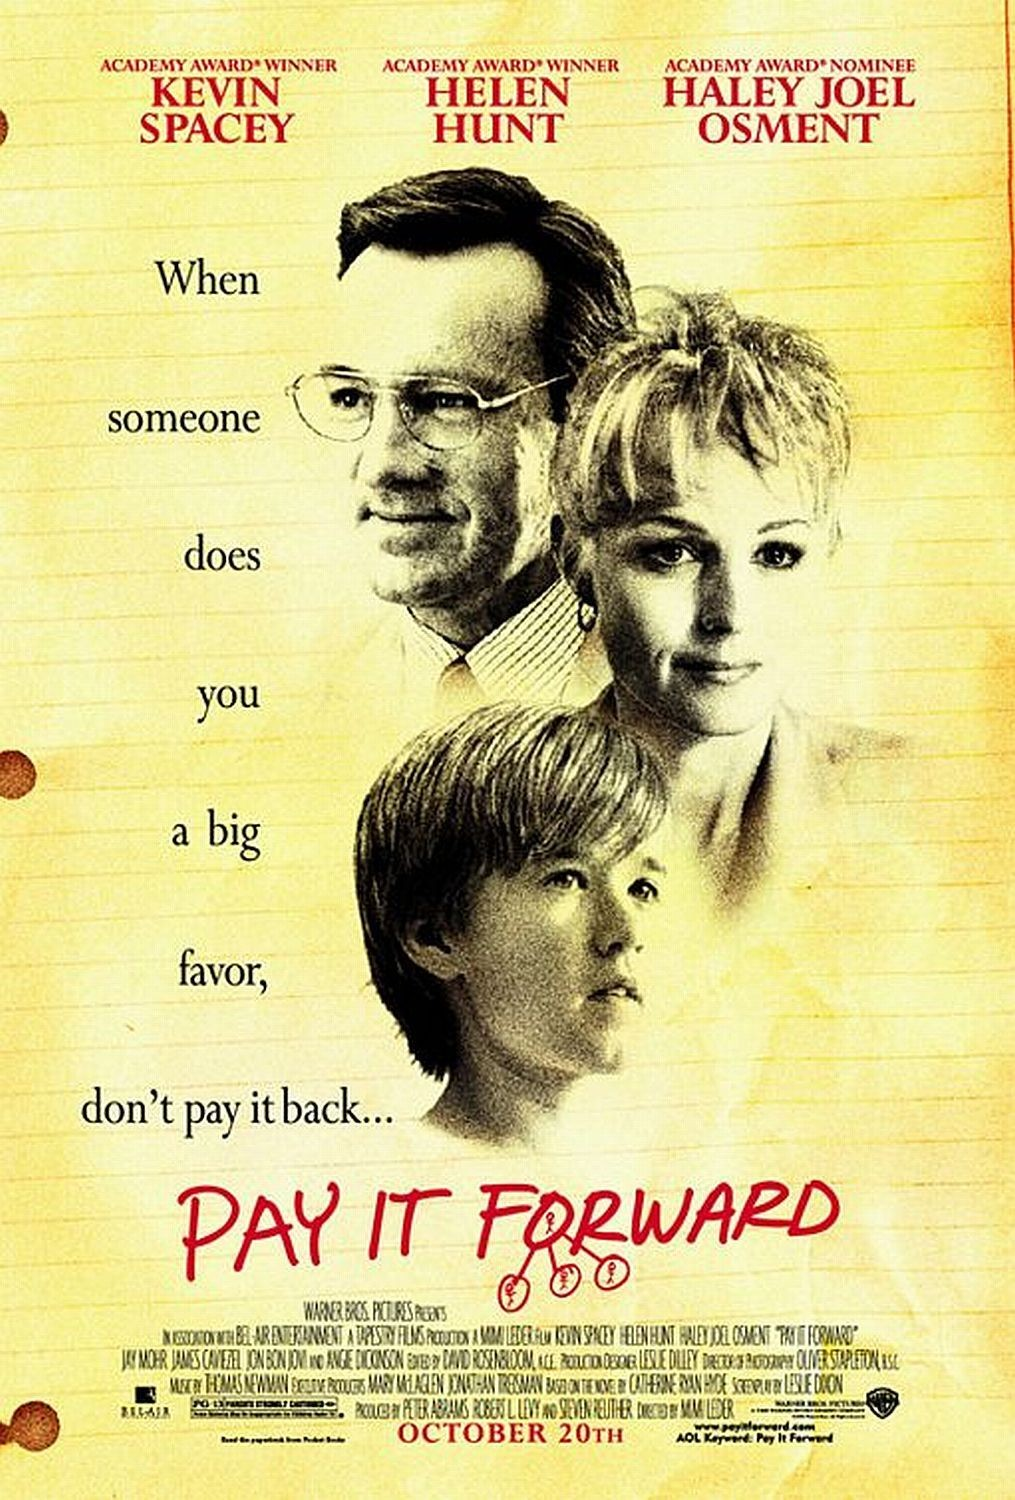
\includegraphics[width=\paperwidth,height=\paperheight]{pay_it_forward}};
% http://tex.stackexchange.com/questions/167719/how-to-use-background-image-in-latex  , figure from wiki:pay_it_forward
\end{document}
